%!TEX root = ../dissertation.tex

\chapter{Evaluation}
\label{chapter:evaluation}
% 1. Present an overview of the evaluation, what we want to evaluate, what we want to conclude.
The present chapter describes the evaluation methodology as also the experiments performed to determine
if a cloud-based approach is adequate to host \gls{RFID} applications middleware. The evaluation process
will focus on establish if such approach can met the low-latecy and scalable data storage requirements
for these applications.\\

Our main goal is to obtain statistical values that allow us to assert if a cloud-based approach is able
to met the expected requirements. With these results, we want to specify which domains can rely in such
approach.

% 2. Present the evaluation methodology for both cases
\section{Evaluation Methodology}
\label{sec:eval_methodology}
In order to determine if a cloud-based \gls{RFID} application is able to met the latency and data
storage scalability requirements, we propose the following methodologies to perform the evaluation:

% Evaluation Methodologies : Data Storage
\subsection{Data Storage Scalability}
\label{sub:eval_methodology_data}
To evaluate the data storage scalability for a \gls{RFID} application based on Fosstrak, the proposed
methodology consists in stress the \gls{EPCIS} Repository by simulating several users that are
concurrently sending events to the repository that is running in the cloud, as illustrated in Figure~\ref{fig:eval_data_methodology}.
The cloud server is running a monitoring system that periodically stores data related to a set of
system metrics, such as \textit{CPU Utilization}, \textit{Network Traffic} and \textit{Memory Usage}.\\

% Data Storage Evaluation Methodology Figure
\begin{figure}[h!]
  \centering
  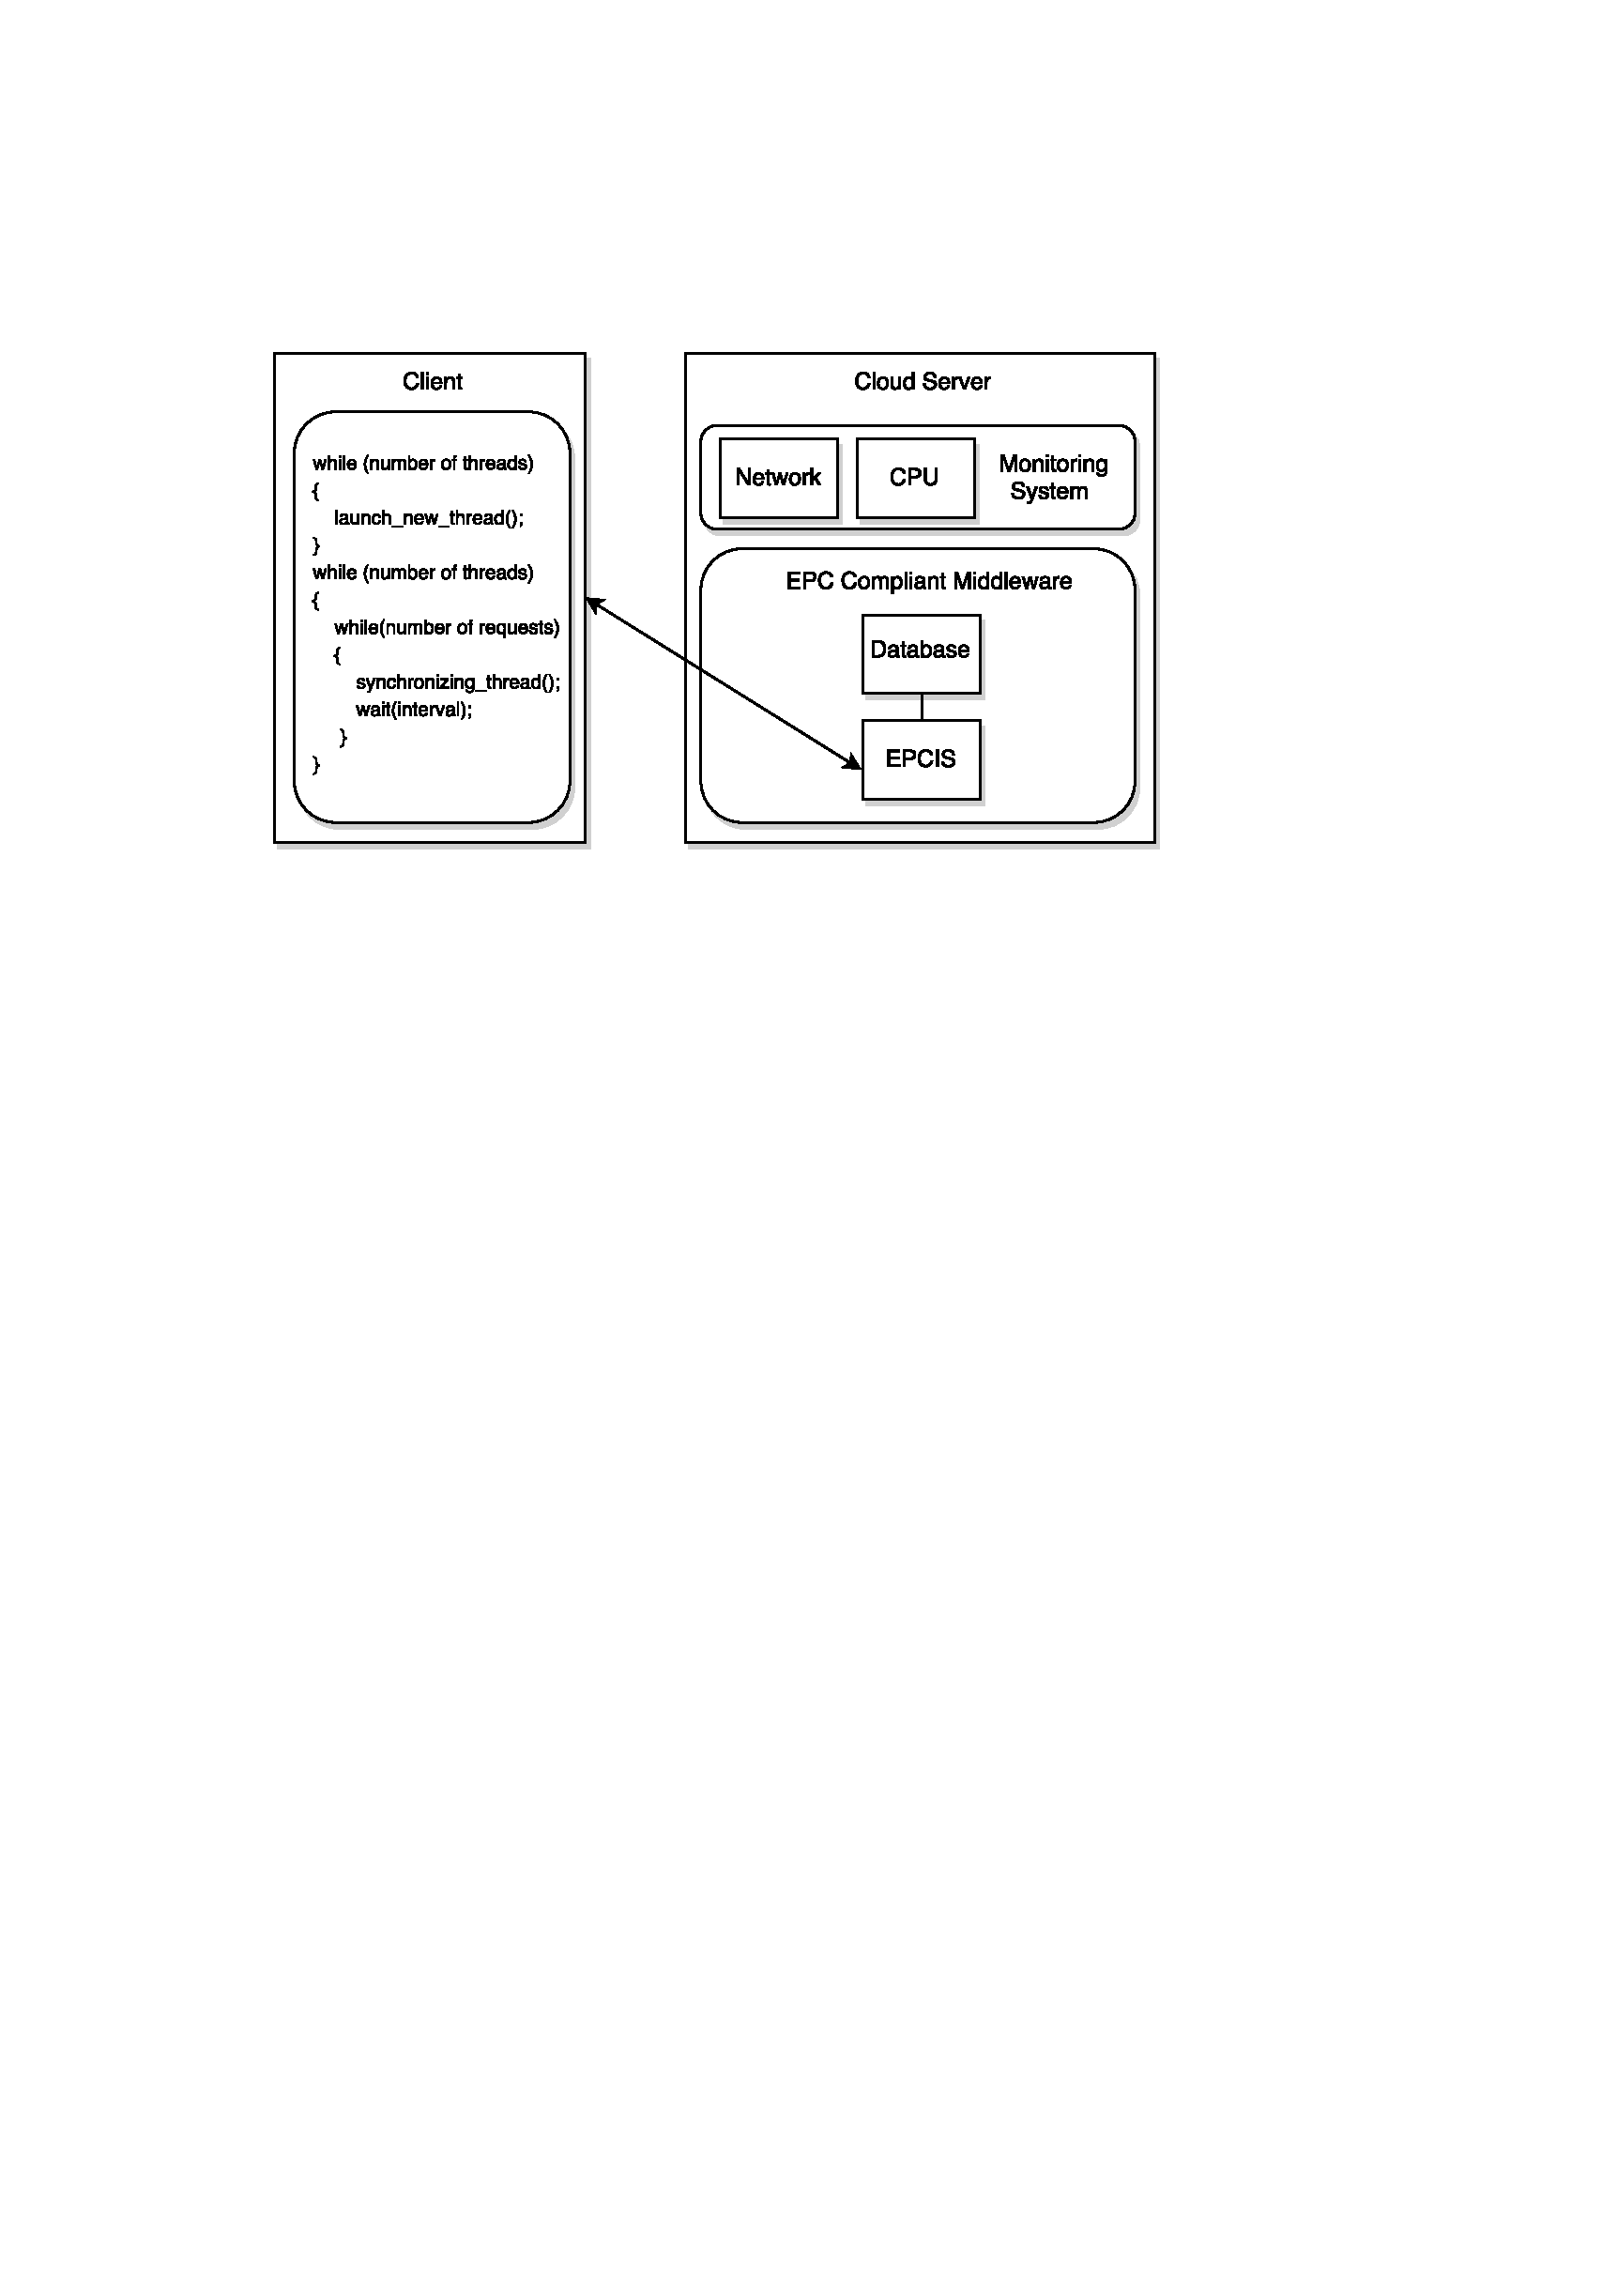
\includegraphics[width=.7\textwidth]{./images/eval_data_methodology}
  \caption{Data Storage Scalability evaluation methodology.}
  \label{fig:eval_data_methodology}
\end{figure}

The analysis of these metrics allows to observe how the performance and behavior of the \gls{EPCIS}
module is affected regarding the amount of events that are processed.

% Evaluation Methodologies : Latency
\subsection{Latency Interaction}
\label{sub:eval_methodology_latency}
To evaluate the latency between an event that occurs in the smart place and the corresponding action
that is triggered, the proposed methodology consists in reproduce a scenario described in Correia et.
al \cite{Correia:Thesis:2014}. In this scenario, a tagged robot was programmed to execute a given number
of laps in a track in which \gls{RFID} readers are placed to detect when the robot is in a given
segment of the track. When the reader detects that a robot is approaching, the reader stores the information
contained in the tag attached in the robot.\\

The Fosstrak \gls{ALE} module is responsible to collect and process the reader events and take the
correct decisions based on these events. In the Fosstrak implementation the collection and processing
of reader events is performed according to an \textit{EventCycle} specification. The \textit{EventCycle}
is a set of periodical read cycles where the \gls{ALE} module collect the events from readers. The data
about the \textit{EventCycle} is delivered to the client through a report. The information in the report
can be used to notify the client regarding a situation in the smart place or even to trigger a new event
in the smart place such as open or close a door.\\

% Latency Interaction Evaluation Methodology Figure
\begin{figure}[h!]
  \centering
  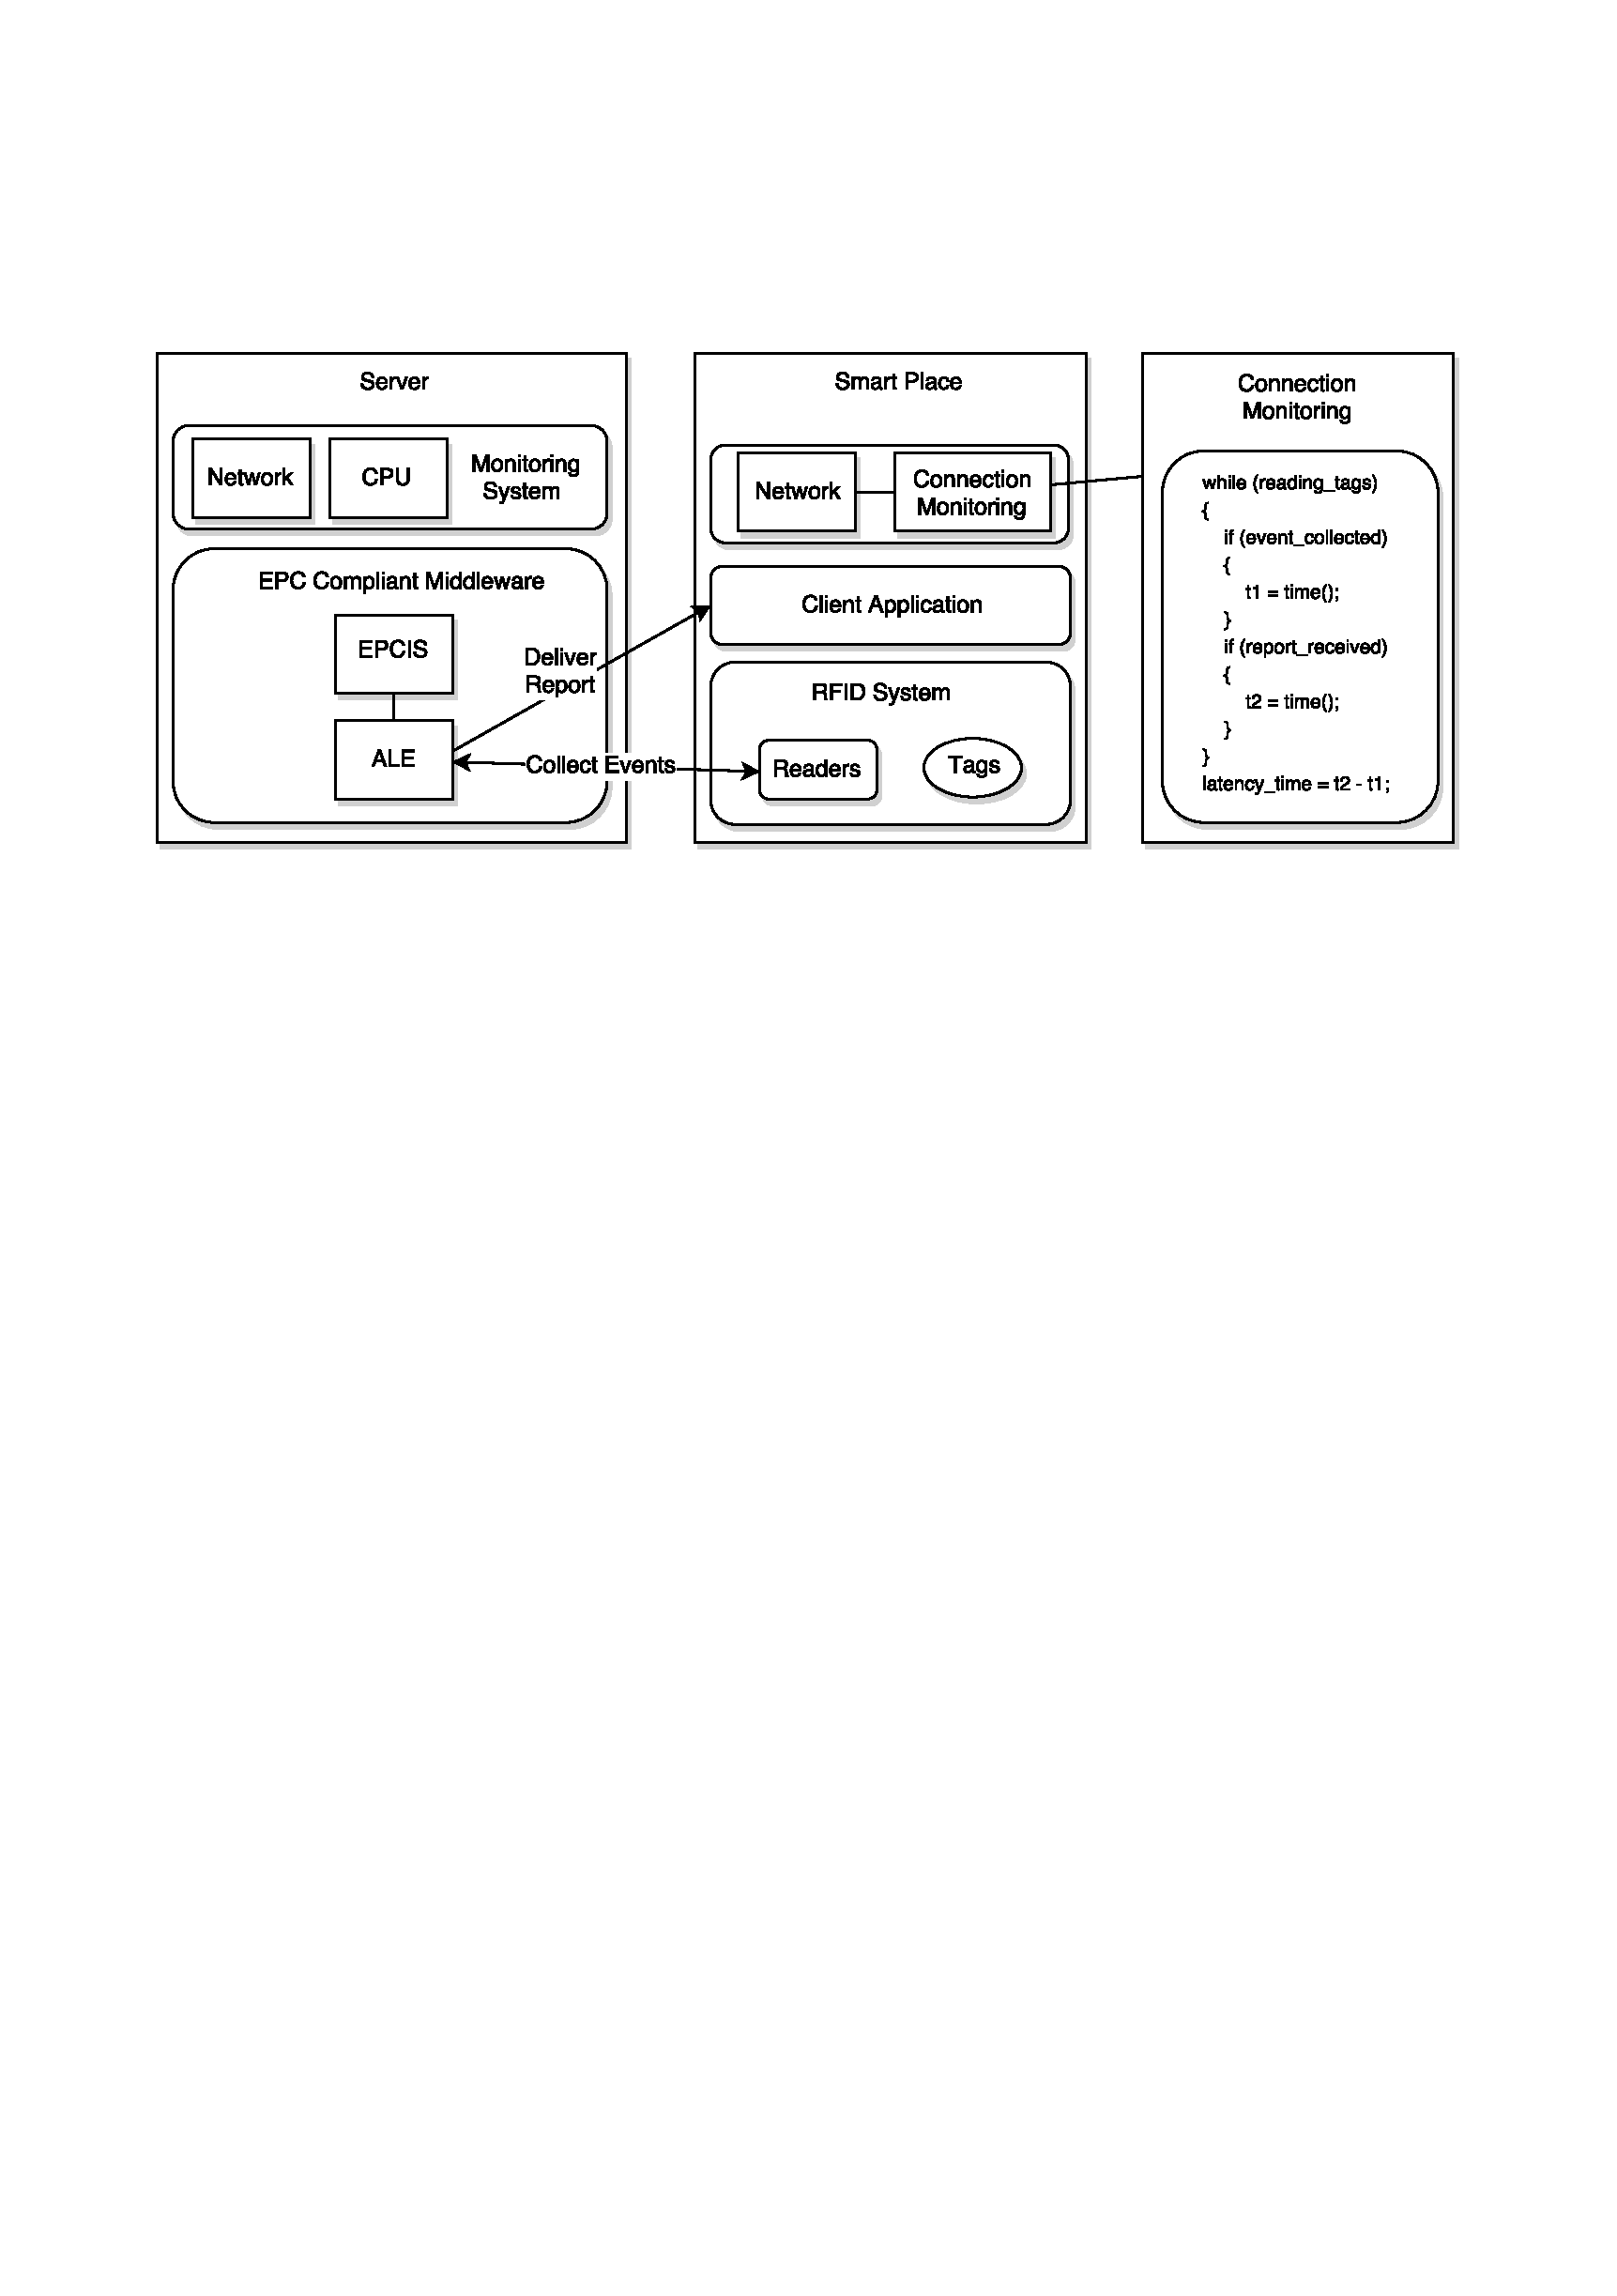
\includegraphics[width=\textwidth]{./images/eval_latency_methodology}
  \caption{Latency interaction evaluation methodology.}
  \label{fig:eval_latency_methodology}
\end{figure}

The smart place is running a monitoring system that stores information about the incoming and outgoing
connections. The Fosstrak \gls{ALE} module can be configured to generate information to register
when a new event is processed and also when the reports are delivered to the clients. Thus, with the
information provided by the monitoring system and the \gls{ALE} module it is possible to calculate
the latency request for an event that occurs in the smart place.\\

With this methodology we intend to obtain information regarding how the communication time is spent
when a event is triggered in the smart place for both approaches described in \ref{}. In order to
determine what approach is more adequate to host the application middleware, the proposed metrics
are considered:

% Metrics
\begin{itemize}
  \item \textit{Event Latency}: the time spent from the moment that an event is triggered in the
  smart place to the moment when the client application receives the notification of the event.
  \item \textit{Upload Latency}: the time spent from the moment that an event is triggered in the
  smart place from the moment when the \gls{ALE} module process the event.
  \item \textit{Response Latency}: the time spent from the moment that the \gls{ALE} module send
  the \textit{Event Cycle} report to the moment that the client receives it.
\end{itemize}

The analysis of those metrics will allow us to compare the performance of both approaches and help to
determine which one is more adequate to host \gls{RFID} applications middleware.

%
% 3. Present the evaluation setup
%
% 4. Present the evaluation scenario (RecPlay Robot case)
%
% 5. Present the performed experiments
%
% 6. Present the result analysis.

%A possible scenario is where a product is being transported from the warehouse inventory section to
%the processing section and there is a door that separates the two sections. When the reader that is
%close to the door detects that a product is approaching the door, an event is triggered and the
%application middleware is responsible to process this event and take the correct decision, in this
%case it must open the warehouse door. In that case we need to determine if a cloud-based solution
%can met the latency interaction requirements for that smart place, otherwise if these requirements are
%not met, a possible situation is where the automated vehicle crashes with door because the request latency
%was to high and then the door took longer to open than expected.\\

% Evaluation Setup
\section{Evaluation Setup}
\label{sec:eval_setup}
To perform the evaluation experiments we choose \gls{AWS} as cloud provider. All the experiments were
conducted in \gls{AWS} \gls{EC2} instances running the Amazon Linux AMI operating system. The virtual
machines presents a configuration with a 2.5\textit{GHz} single-core processor with 1\textit{Gb} of
RAM. In the configuration where the \gls{ALE} module is provisioned in the smart place, the experiments
were conducted in a virtual machine with a 2.6\textit{GHz} dual-core processor with 2\textit{Gb} of
RAM and running the \textit{Linux Ubuntu 14.04.1 LTS} operating system. Regarding the \gls{RFID}
readers, the Rifidi Emulator\footnote{http://rifidi.org} was used to emulate the physical readers
that are in the smart place.\\

Regarding software components, the application stack is composed of the \textit{Apache Tomcat 7.0.52.0}\footnote{http://tomcat.apache.org/}
with \textit{Java} version \textit{1.7.0} update \textit{79}. The \gls{RFID} middleware used was the Fosstrak
described in section \ref{sub:fosstrak}. The middleware stack is available at the Fosstrak’s\footnote{http://fosstrak.github.io/}
source control system, and the versions were: a) \textit{FCServer} version \textit{1.2.0}; b) \textit{Capture Application}
version \textit{0.1.1}; and c) \textit{\gls{EPCIS} Repository} version \textit{0.5.0}. Furthermore,
the \gls{EPCIS} Repository was connected to a \textit{MySQL server} version \textit{5.5} that stores
all the \gls{EPCIS} events.

% Evaluation Experiments
\section{Evaluation Experiments}
\label{sec:eval_experiments}

% Evaluation Analysis
\section{Evaluation Analysis}
\label{sec:eval_analysis}
